\documentclass[a4paper,20pt]{article}
\usepackage{amsmath,amssymb,epsf,epsfig,times}
\usepackage{multicol}
\usepackage[all]{xy}
\usepackage{color}
\usepackage{ctex}
\usepackage{subfigure}
\usepackage{url,cite}
\usepackage{tikz}
\usepackage[english]{babel}
\usepackage[utf8]{inputenc}

\usepackage{pdfpages}

%\usepackage{caption}
%
%\usepackage[font=small,labelfont=bf,labelsep=none]{caption}
\usepackage[font=default,labelfont=bf,labelsep=period]{caption}

\usepackage{makecell}
\usepackage{booktabs} %引入三线表
\usepackage{diagbox}
\usepackage{multirow}

\usepackage{fancyhdr}
\usepackage{float}
\usepackage{ulem}

\usepackage{listings}
\usepackage{xcolor}

\usepackage{enumerate}
\lstset{
    basicstyle          =   \sffamily,          % 基本代码风格
    keywordstyle        =   \bfseries,          % 关键字风格
    commentstyle        =   \rmfamily\itshape,  % 注释的风格,斜体
    stringstyle         =   \ttfamily,  % 字符串风格
    flexiblecolumns,                % 别问为什么,加上这个
    numbers             =   left,   % 行号的位置在左边
    showspaces          =   false,  % 是否显示空格,显示了有点乱,所以不现实了
    numberstyle         =   \zihao{-5}\ttfamily,    % 行号的样式,小五号,tt等宽字体
    showstringspaces    =   false,
    captionpos          =   t,      % 这段代码的名字所呈现的位置,t指的是top上面
    frame               =   lrtb,   % 显示边框
}
\lstdefinestyle{Python}{
    language        =   Python, % 语言选Python
    basicstyle      =   \zihao{-5}\ttfamily,
    numberstyle     =   \zihao{-5}\ttfamily,
    keywordstyle    =   \color{blue},
    keywordstyle    =   [2] \color{teal},
    stringstyle     =   \color{magenta},
    commentstyle    =   \color{red}\ttfamily,
    breaklines      =   true,   % 自动换行,建议不要写太长的行
    columns         =   fixed,  % 如果不加这一句,字间距就不固定,很丑,必须加
    basewidth       =   0.5em,
}

\newtheorem{theorem}{Theorem}[section]
\newtheorem{lemma}{Lemma}[section]
\def\proof{\noindent{\it Proof: }}
\def\QED{\mbox{\rule[0pt]{1.5ex}{1.5ex}}}
\def\endproof{\hspace*{\fill}~\QED\par\endtrivlist\unskip}
\newcommand{\re}{\mathbb{R}}
\def\sV{\mathcal{V}}
\def\sS{\mathcal{S}}
\def\sQ{\mathcal{Q}}

\newcommand{\mc}{\mbox{: }}

\newcommand{\normsq}[1]{\left\|#1\right\|^2}
\newcommand{\norm}[1]{\left\|#1\right\|}
%\newcommand{\sgn}[1]{\mbox{sgn}(#1)}
\newcommand{\pde}[2]{\frac{\partial #1}{\partial #2}}
\newcommand{\fundef}[3]{#1:#2\to #3}
\newcommand{\abs}[1]{\left|#1\right|}
\newcommand{\mymatrix}[2]{\left(\begin{array}{#1}#2\end{array}\right)}
\newcommand{\defeq}{\stackrel{\triangle}{=}}
\newcommand{\paren}[1]{\left(#1\right)}
%\theoremstyle{plain} \newtheorem{theorem}{Theorem}
%\theoremstyle{plain} \newtheorem{algorithm}{Algorithm}
\newtheorem{axiom}[theorem]{Axiom}
\newtheorem{definition}[theorem]{Definition}
\newtheorem{assumption}[theorem]{Assumption}
\newtheorem{example}[theorem]{Example}
%\theoremstyle{plain}\newtheorem{lemma}{Lemma}
%\newtheorem{proposition}[theorem]{Proposition}
\newtheorem{remark}[theorem]{Remark}
\newtheorem{corollary}[theorem]{Corollary}

\newcommand{\Acal}{\mathcal{A}}
\newcommand{\Bcal}{\mathcal{B}}
\newcommand{\Ccal}{\mathcal{C}}
\newcommand{\Dcal}{\mathcal{D}}
\newcommand{\Ecal}{\mathcal{E}}
\newcommand{\Fcal}{\mathcal{F}}
\newcommand{\Gcal}{\mathcal{G}}
\newcommand{\Hcal}{\mathcal{H}}
\newcommand{\Ical}{\mathcal{I}}
\newcommand{\Jcal}{\mathcal{J}}
\newcommand{\Kcal}{\mathcal{K}}
\newcommand{\Lcal}{\mathcal{L}}
\newcommand{\Mcal}{\mathcal{M}}
\newcommand{\Ncal}{\mathcal{N}}
\newcommand{\Ocal}{\mathcal{O}}
\newcommand{\Pcal}{\mathcal{P}}
\newcommand{\Qcal}{\mathcal{Q}}
\newcommand{\Rcal}{\mathcal{R}}
\newcommand{\Scal}{\mathcal{S}}
\newcommand{\Tcal}{\mathcal{T}}
\newcommand{\Ucal}{\mathcal{U}}
\newcommand{\Vcal}{\mathcal{V}}
\newcommand{\Wcal}{\mathcal{W}}
\newcommand{\Xcal}{\mathcal{X}}
\newcommand{\Ycal}{\mathcal{Y}}
\newcommand{\Zcal}{\mathcal{Z}}


\def\omegavec{\boldsymbol{\omega}}
\newcommand{\alphabf}{\boldsymbol{\alpha}}
\newcommand{\omegabf}{\boldsymbol{\omega}}
\def\omegavec{\boldsymbol{\omega}}
\newcommand{\taubf}{\boldsymbol{\tau}}
\newcommand{\qbf}{\mathbf{q}}
\newcommand{\ybf}{\mathbf{y}}
\newcommand{\pbf}{\mathbf{p}}
\newcommand{\rbf}{\mathbf{r}}
\newcommand{\ebf}{\mathbf{e}}
\newcommand{\onebf}{\mathbf{1}}
\newcommand{\zerobf}{\mathbf{0}}
\newcommand{\abf}{\mathbf{a}}
\newcommand{\ibf}{\mathbf{i}}
\newcommand{\jbf}{\mathbf{j}}
\newcommand{\kbf}{\mathbf{k}}
\newcommand{\vbf}{\mathbf{v}}
\newcommand{\wbf}{\mathbf{\omega}}
\newcommand{\fbf}{\mathbf{f}}
\newcommand{\zbf}{\mathbf{z}}
\newcommand{\xbf}{\mathbf{x}}
\newcommand{\dbf}{\mathbf{d}}
\newcommand{\Rbf}{\mathbf{R}}
\newcommand{\Tbf}{\mathbf{T}}

\newcommand{\Cbf}{\mathbf{C}}
\newcommand{\Ibf}{\mathbf{I}}
\newcommand{\Pbf}{\mathbf{P}}
\newcommand{\Qbf}{\mathbf{Q}}
\newcommand{\Vbf}{\mathbf{V}}
\newcommand{\Jbf}{\mathbf{J}}
\newcommand{\Xbf}{\mathbf{X}}
\newcommand{\Abf}{\mathbf{A}}
\newcommand{\Kbf}{\mathbf{K}}
\newcommand{\Gammabf}{\boldsymbol{\Gamma}}
\newcommand{\nubf}{\boldsymbol{\nu}}
\newcommand{\xibf}{\boldsymbol{\xi}}
\newcommand{\Xibf}{\boldsymbol{\Xi}}
\newcommand{\Omegabf}{\boldsymbol{\Omega}}


\newcommand{\ubf}{\mathbf{u}}

\newcommand{\lth}{\ell{\text{th}}}
\newcommand{\ith}{i{\text{th}}}
\newcommand{\jth}{j{\text{th}}}
\newcommand{\kth}{k{\text{th}}}
\newcommand{\ip}[2]{\left<#1,~#2\right>}

\newcommand{\OMIT}[1]{}
\title{}
\author{}
\date{}


\pagestyle{fancy}
\fancyhf{}
\chead{\textbf{关于$\lceil$\textcolor{red}{“非线性规划”}$\rfloor$的matlab讲解}}
\lhead{魔力铠甲}
\rfoot{Page \thepage}
\begin{document}
\renewcommand{\lstlistlistingname}{代码汇总}
\renewcommand{\lstlistingname}{代码}
\captionsetup[figure]{labelfont={bf},labelformat={default},labelsep=period,name={图}}
\renewcommand\tablename{表}
\begin{itemize}
    \item[1.]编码请看Homework1.m与deltaf.m.
    \\极值点是$x_1=0.3333,x_2=1.3333$
    \\极值是$Z=4.6667$
    \item[2.]编码请看Homework2.m与nwfun.m.(此时步长为1)
    \\极值点是$x=0,y=0$
    \\极值是$Z=-0.5$(迭代408次)
    \\另一个编码请看c\_gradientDescent.m(此时步长可变)
    \\极值点是$ x=10^{-4}*0.1002,y=0$
    \\极值是$Z=-0.5$(迭代100次左右)
    \item[3.]   数学模型为:
        \par \noindent $\min f(x)=0.2(x_1^2+x_2^2+x_3^2)+58x_1+54x_2+50x_3-560$
        \\s.t.$\left\{\begin{matrix}
                x_1+x_2+x_3=180    \\
                x_1+x_2\geq 100    \\
                x_1 \geq 40        \\
                x_1,x_2,x_3 \geq 0 \\
            \end{matrix} \right.$
        \\给出非线性规划的解:   $x_1=40
            \quad x_2=60
            \quad x_3=80$
        \\$fval =1.0160*10^{4}$
    \item[4.] 给出解,代码详见homework4.m,Objfun41.m与Confun41.m
        \\$x =\quad  0.0000  \quad  0.0000  \quad  2.7977 \quad  -0.0001  \quad  0.0000  \quad  0.9321$
    \item[5.] 解同4,留给读者。
    \item[6.] 给出fmincon的解,代码详见homework6.m,Objfun61.m与Objfun62.m:
        \\$x =\qquad    2.3333 \qquad   0.1667 \qquad  -3.4444$
            \\$fval =\qquad  -18.0833 $
    \item [7.]假设题目给出的已知参数是合理的。同时已知电影院的座位应该是离散的,人的眼睛位于人的座位的正上方,不考虑眼距,屏幕在水平方向上的大小等。
          \par \noindent (1).我们假设所分析的对象的满意度是$f(\alpha,\beta)=g(\alpha)-h(\beta)$,其中令g,h都是最简单的形式;也就是说,不妨设
          \\$g(\alpha)=\alpha,h(\beta)=\left\{\begin{matrix}
              0,\beta\leq 30^\circ      \\
              \beta,\beta \geq 30^\circ \\
          \end{matrix}\right.$
              \\然后我们假设观影院屏幕所在为y轴,水平地面为x轴,建立坐标系并分析:
              \\我们对其上一点人设为(x,y);随后有$d\leq x \leq D$,并且满足$y=\tan(\theta)(x-d)$
              \\从而人的视角有方程$y^*=\tan(\theta)(x-d)+c$
              \\建立对$\alpha$与$\beta$的分析,由斜率和三角函数关系可知:
              \begin{center}
                  $\alpha=\arctan\left(\frac{|\frac{y^*-H}{x}-\frac{y^*-H+h}{x}|}{1+\frac{y^*-H}{x}\cdot \frac{y^*-H+h}{x}} \right)$
              \end{center}
              $$ \beta = \arctan\left(\frac{y^*-H}{x}\right)$$
              \par \noindent 随后便可以根据两个方程对x进行作图。
              \\根据图片不难看出,在不考虑$\beta \geq 30^\circ$的境况下,
              \\$\alpha$随着x的增加而减少,此时很显然推荐的座位便是距离屏幕水平距离6.111距离处的位置。
          \begin{figure}[h]
              \centering
              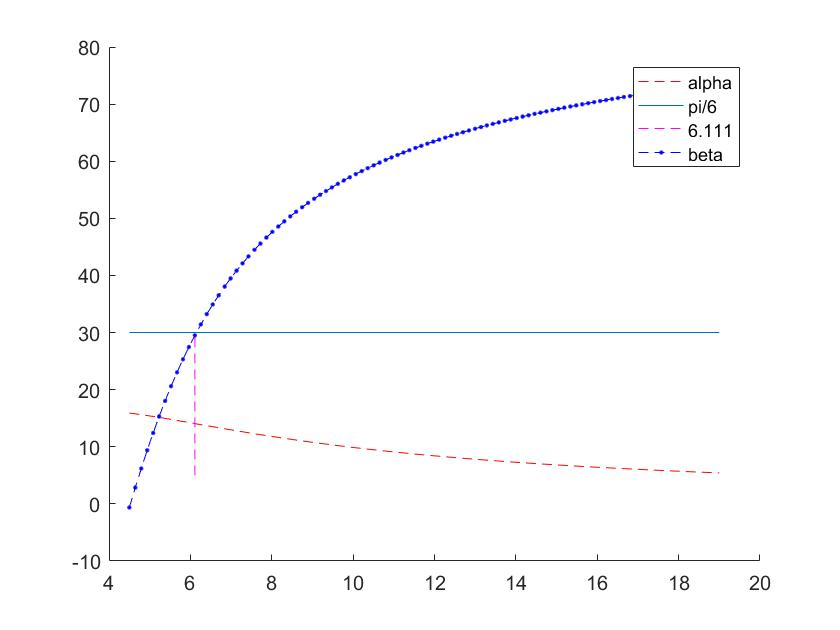
\includegraphics[width=300pt,height=170pt]{Homework7_1.jpg}
              \caption{第一问假设}
          \end{figure}
          \par \noindent (2).我们假设满意度最大的时候就是$\alpha$最大的时候。
          \begin{figure}[h]
              \centering
              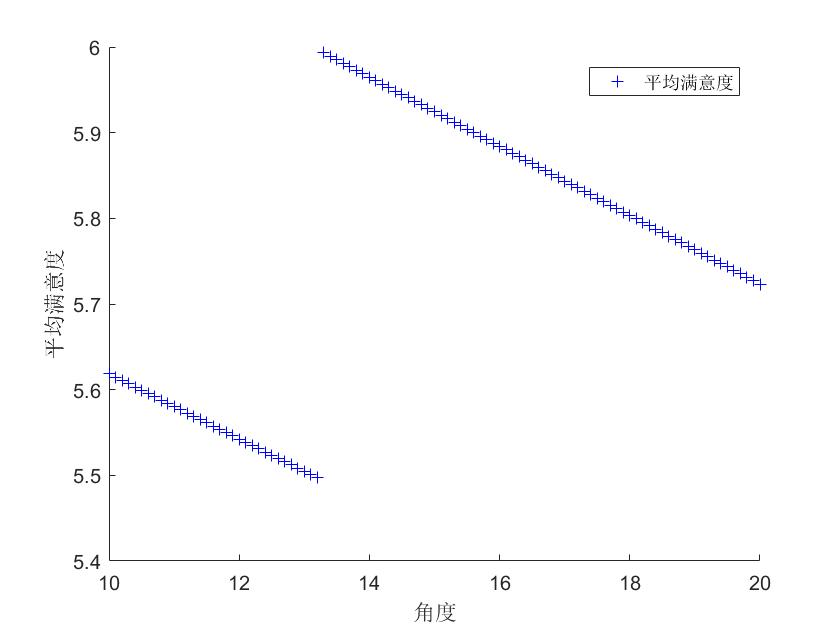
\includegraphics[width=300pt,height=170pt]{Homework7_2.jpg}
              \caption{第二问假设}
          \end{figure}
          \par \noindent 那么$\theta=13.75^\circ$时观众平均满意度最大。
          \par \noindent 对于每个固定的x,如果将观众的位置在y方向上提高,经过简单的画图分析提高座位高度可一定程度上提高某个位置的满意度。用模型一来探究高度对平均满意度的影响,此时为简便假设θ取第二问中求得的最佳角度。
          在前面的讨论中地板线均是直线,那么考虑折线是否能提高满意度。首先可以先选取合适的一排z,在z之前不变,在z这一排又建立关系重新设定不同的角度。
          \begin{figure}[h]
              \centering
              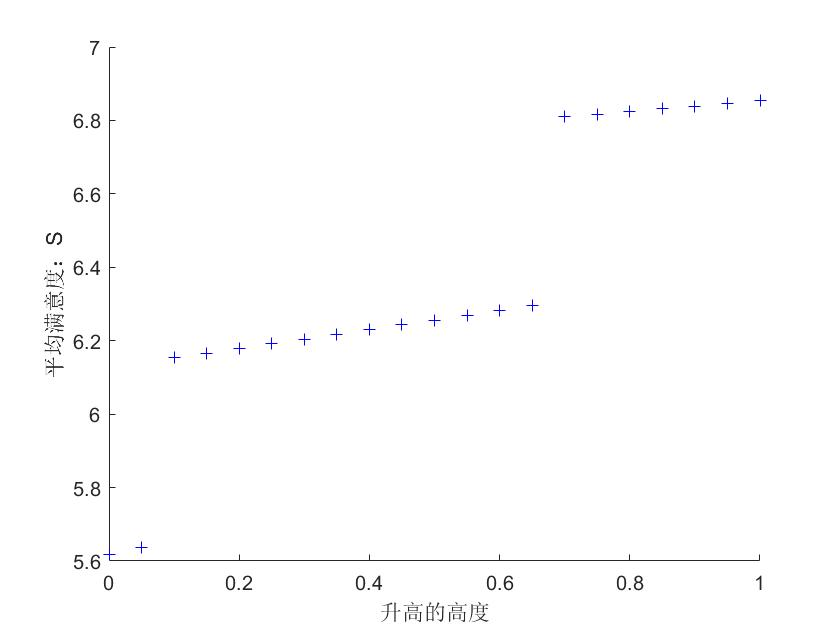
\includegraphics[width=300pt,height=170pt]{Homework7_3.jpg}
              \caption{第三问假设}
          \end{figure}
          \par \noindent 所以可以升高座位大概 6.5cm左右。
\end{itemize}
\end{document}